
%%%%%%%%%%%%%%%%%%%%%%% file typeinst.tex %%%%%%%%%%%%%%%%%%%%%%%%%
%
% This is the LaTeX source for the instructions to authors using
% the LaTeX document class 'llncs.cls' for contributions to
% the Lecture Notes in Computer Sciences series.
% http://www.springer.com/lncs       Springer Heidelberg 2006/05/04
%
% It may be used as a template for your own input - copy it
% to a new file with a new name and use it as the basis
% for your article.
%
% NB: the document class 'llncs' has its own and detailed documentation, see
% ftp://ftp.springer.de/data/pubftp/pub/tex/latex/llncs/latex2e/llncsdoc.pdf
%
%%%%%%%%%%%%%%%%%%%%%%%%%%%%%%%%%%%%%%%%%%%%%%%%%%%%%%%%%%%%%%%%%%%


\documentclass[runningheads,a4paper]{llncs}

\usepackage{amssymb}
\setcounter{tocdepth}{3}
\usepackage{graphicx}

\usepackage{url}
\urldef{\mailsa}\path|{caldwelt, david.t.coleman, nikolaus.correll}@colorado.edu|    
\newcommand{\keywords}[1]{\par\addvspace\baselineskip
\noindent\keywordname\enspace\ignorespaces#1}

\usepackage{color}
\usepackage{wrapfig}


\begin{document}

\mainmatter  % start of an individual contribution

% first the title is needed
\title{Robotic Manipulation for Identification of Flexible Objects}

% a short form should be given in case it is too long for the running head
\titlerunning{Robotic Manipulation for Identification of Flexible Objects}


\author{T. M. Caldwell and  D. Coleman and N. Correll%
\thanks{
This work was supported by a NASA
Early Career Faculty fellowship NNX12AQ47GS02. We are grateful for this support.}%
}
%
\authorrunning{Robotic Manipulation for Identification of Flexible Objects}
% (feature abused for this document to repeat the title also on left hand pages)

% the affiliations are given next; don't give your e-mail address
% unless you accept that it will be published
\institute{Department of Computer Science, University of Colorado,\\
1111 Engineering Dr, Boulder, CO 80309, USA\\
\mailsa}

\toctitle{Lecture Notes in Computer Science}
\tocauthor{Authors' Instructions}
\maketitle

\section{Motivation, Problem Statement, Related Work}
\begin{wrapfigure}{r}{0.4\textwidth}
\centering
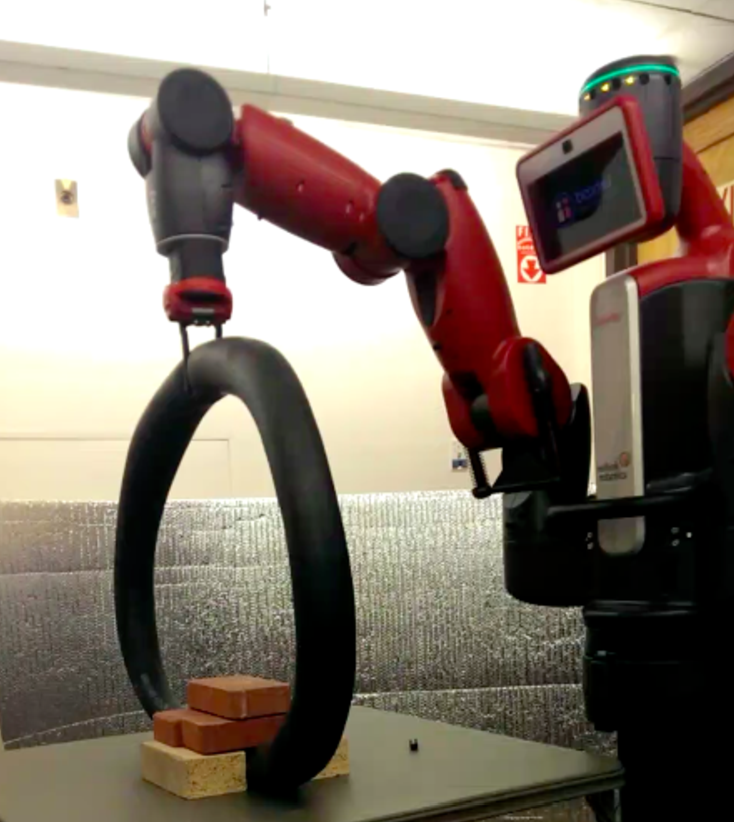
\includegraphics[width = 0.37\textwidth]{baxter_experiment_image}
\caption{Rethink Robotics' Baxter manipulating an inflated bicycle tyre.}
\label{fig-baxter_image_1}
\end{wrapfigure}

% 1. What do you want to do
When a robot initially interacts with a flexible object with unknown properties, the robot must first manipulate the object, possibly in a naive manner in order to ascertain characteristics for future manipulation.  The goal of this work is to use a robotic arm to identify the behavior of flexible objects through manipulation, where we emphasis measurements through touch. This is an important step toward manipulation of flexible objects such as rubber tubes, plants or clothes  \cite{bell2010flexible} \cite{jimenez2012survey} \cite{saha2007manipulation} \cite{wakamatsu2006knotting}.  
% 2. How is it done now and what are the limitations of current practice

There are many methods to model and simulate flexible objects \cite{khalil_payeur} \cite{lang_etal}.  A common approach is to model the object as a lattice or collection of links of masses and springs \cite{sahari_etal} \cite{wakamatsu_etal}  \cite{khalil_payeur}.  This approach has been used to simulate linear object like strings, hair, and electrical cables for which the model is a series of masses linked together with springs. %%% MISSING: LIMITATIONS OF THIS APPROACH  

% 3. What are you doing that is new and why do you think it will be successful
%Our approach is similar with the primary difference that the loop connects back onto itself.  This connection restricts the loops movement and is handled using holonomic constraints.  To the best of our knowledge, no one has used a robot to identify parameters of a flexible loop for manipulation.

This work is a continuation of \cite{caldwell_coleman_correll} in which we used the Baxter robot in Fig~\ref{fig-baxter_image_1} to identify the stiffness properties of a rubber loop.  While bending, twisting, and stretching the loop, the robot measures the arm's joint torques and joint angles.  We used an optimal estimation approach to find the stiffness properties of a model that best matches the measurement.  Refer to the paper for details on the model and optimization procedure.

This paper validates the parameter identification through additional experiments and the use of an additional arm.  The paper's primary technical details are concerned with merging the data from these experiments.

%\begin{enumerate}
%\item I see this paper as a ``roadmap paper''.  Sort of these are the challenges, this is how we plan to solve them, and there are a lot of interesting problems.
%\item Problem statement: ``When a robot initially interacts with a flexible object with unknown properties, the robot must first manipulate the object, possibly in naive, unstructured manner in order to ascertain characteristics for future purpose driven manipulation.''
%\item Proper identification has a number of challenges:
%\begin{enumerate}
%  \item Integrate touch with visual sensors.
 % \item Where/how to initially grip the object.
 % \item Multiple grip locations and multiple tests for identification.
 % \item Multiple arms.
 % \item Additional stimuli like external forces that are due to other objects than the one of consideration---for example, working in a cluttered environment.
%  \item Choosing manipulator trajectories that provide the most information.
 % \item Unknown topology or geometry
 % \item Choosing the model discretization that best balances model fidelity with computation speed.
%  \item Stable manipulation while maintaining fidelity of parameter optimization
 % \item Updating identification for systems that will change over long time horizon's---for example plant growth over full life cycle.
%\end{enumerate}
%\item Related Work:
%\begin{enumerate}
 % \item There are many methods to model and simulate flexible objects \cite{khalil_payeur} \cite{lang_etal}.  A common approach is to model the object as a lattice or collection of links of masses and springs \cite{sahari_etal} \cite{wakamatsu_etal} \cite{khalil_payeur}.
%  \item  Alternatively, the cost can be given by a maximum likelihood estimate for which the cost is lower for parameters that correspond to the simulation that is most consistent with the measurement (see \cite{houska_etal}).  
%\end{enumerate}
%\item What's new?---``Our approach is similar with the primary difference that the loop connects back onto itself.  This connection restricts the loops movement and is handled using holonomic constraints.  To the best of our knowledge, no one has used a robot to identify parameters of a flexible loop for manipulation.''
%\item Who cares?:
%\item What difference will it make?---Advancing autonomy of robotic systems.
%\item Risks/payoffs?---Additional time and computation to analyze object compared to solely reactive manipulation \textbf{cite}, but once accomplished, model-based planning can be done, which is even more important for potentially unstable manipulation.
%\end{enumerate}


\section{Technical Approach}
\label{sec-tech}
The problem of optimal parameter identification of a flexible object through multiple experiments has three primary technical challenges:
\begin{enumerate}
\item the object's model,
\item the optimization procedure, and 
\item consolidating the identification through multiple experiments.
\end{enumerate}

In \cite{caldwell_coleman_correll}, we model the robot's interaction with the flexible object using variational integrators.  Variational integrators can be used to describe the discrete-time equations of motion of a mechanical system.  They are designed from the least action principle and have good properties that agree with known physical phenomenon like stable energy behavior \cite{pekarek_murphey}.  In addition, they handle holonomic constraints directly which are needed for objects that loop back on themselves and for multiple grasp points by the robotic arm. 

Furthermore, in \cite{caldwell_coleman_correll}, we set up the parameter identification optimization problem as a discrete-time Bolza problem where we provided a discrete-time adjoint-based gradient calculation the cost functional with respect to the parameters.  The gradient is needed for derivative-based optimization procedures like steepest descent and Newton's method to identify the optimal parameters.  In this paper, we wish to extend this single experiment approach to multiple experiments in order to increase the confidence of the parameter measurement.  In the full paper, we formalize the following algorithm for consolidating the identification from multiple experiments.  
\begin{enumerate}
\item Choose initial parameters $\rho_0$ and initial confidence $c_0$ for those parameters.  Set $k = 1$.
\item Design the $k^\textrm{th}$ experiment to be distinct from all previous.
\item Run the $k^\textrm{th}$ experiment and record relevant measurements $y_{k}$.
\item Calculate optimal parameters $\rho_k$ given $\rho_{k-1}$, $y_{k}$ and $c_k$.
\item Increment $k$.
\item Repeat from step 2 until $c_k$ reaches a desired value, in which case return identified parameters $\rho_{k}$ with confidence $c_k$.
\end{enumerate}
The details and analysis of each step in the algorithm, as well as the confidence value $c_k$ are in the full paper.  

%\begin{enumerate}
%\item Model based approach---``In this paper, the manner in which we model the loop is so that the underlying mechanics of the loop are the same as the robot arm, i.e., a collection of rigid bodies connected by springs, allowing us to utilize the vast theory of rigid body mechanics \cite{murray_li_sastry}.''
%\item Planning and control for full robot/object system---``this enables planning and control to be done in the combined arm and loop configuration space instead of the end effector or object space.''
%\item Optimal parameter identification---``optimal control approach for calculating model properties that best match the behavior of the physical loop.''
%\begin{enumerate}
%\item Setup---``The parameter identification optimization problem is set up as a discrete-time Bolza problem.  For the loop example, the cost functional is a summation of the error between the simulated end effector position and the experimentally-measured end effector position.  The joint error directly correlates to the difference between the simulated loop displacement and the measured loop displacement, at least at the manipulator.''
%\item The problem---``For the discrete problem, it is reasonable to choose a discrete cost functional that approximates the continuous cost\textemdash i.e. $\ell_d(x_{k},\rho)\approx\int_{t_{k-1}}^{t_{k}}\ell(x(\tau),\rho)d\tau$ and $m_d(x_{k_f},\rho)\approx m(x(t_f),\rho)$.  Alternatively, $\ell_d$ and $m_d$ can be designed directly without first choosing an underlying continuous cost.  The discrete parameter optimization problem is as follows:
%The integration could be approximated with a quadrature like midpoint rule.  Additionally, in order to use the one-step mapping Eq.(\ref{eq-fk}) and its linerization, Eqs.(\ref{eq-A}) and (\ref{eq-B}), we transform the pair $(q_{k-1},q_k)$ to $(q_k,p_k)=:x_k$ using Eq.(\ref{eq-pk}) so that the discrete running cost instead depends on the state\textemdash i.e. $\ell_d(x_k,\rho)$.  In a similar manner, the discrete terminal cost is chosen to approximate continuous terminal cost\textemdash i.e. $m_d(x_{k_f},\rho)\approx m(x(t_f),\rho)$.  The discrete parameter optimization problem is as follows:
%\begin{problem}[Discrete System Parameter Optimization]
%Calculate the parameters $\rho\in\mathcal{P}$ which solves:
%\[
%\min_{\rho\in\mathcal{P}} \Big[J_d(\rho):=\sum_{k=1}^{k_f}\ell_d(x_k,\rho) + m_d(x_{k_f},\rho)\Big]
%\]
%constrained to $x_{k+1} = f(x_k,\rho,t_k)$, Eq.(\ref{eq-fk}).
%\label{prob-disc}
%\end{problem}
%''
%\item The Approach---``In optimal control theory, it is common practice to solve optimization problems using iterative methods.  Iterative optimization methods repeatedly reduce the cost by stepping in a descending direction until a local optimum is found.  Commonly, the step direction and step size is calculated using local derivative information \cite{armijo}\cite{kelley}, which is practiced in this paper.''
%\item Gradient---Lemma 1 from paper
%\end{enumerate}
%\item Using variational integrators---``A good representation of a flexible object is not enough to accurately model it.  We also need the model simulation to be consistent with the physical behavior of the loop.''
%\begin{enumerate}
 % \item Generalized Coordinates---``Due to recent work by Johnson and Murphey \cite{johnson_murphey_scalable} \cite{johnson_murphey_linearization}, it is possible to efficiently simulate mechanical systems using variational integrators in generalized coordinates. They provide a framework using a tree representation and caching that not only makes for efficient simulation---especially for articulated rigid bodies''
%  \item Has good physical properties---``We decided not to apply Euler integration or another low order integrator to the continuous dynamics, as is the case in \cite{sahari_etal}, because such integrators can introduce significant energy errors.  At worst these errors will destabilize the integration and at best compromise the model's energy dissipation \cite{johnson_murphey_scalable}. Instead we decided to use \emph{variational integrators}.  Variational integrators can be used to describe discrete-time equations of motion of a mechanical system.  They are designed from the least action principle and have good properties that agree with known physical phenomenon like stable energy behavior \cite{pekarek_murphey}.''
  %\item Holonomic constraints---``variational integrators elegantly handle holonomic constraints.  Holonomic constraints are specified as $h(q) = 0$, where $q$ is the system's configuration.  They are used to constrain positions and orientations.  For the example, we use holonomic constraints to ``close the loop''---i.e. to constrain the link at one end of the loop to the other end.  In simulating continuous dynamics, holonomic constraints are commonly handled with equivalent constraints on the acceleration that can creep due to numerical integration error.  In comparison, variational integrators apply holonomic constraints directly and do not have this issue (see \cite{johnson_murphey_scalable} for a discussion).''
%  \item Model based calculations---``efficient model-based calculations like linearizations about a trajectory.   In optimal controls, linearizations are needed for gradient calculations like the gradient calculation presented in this paper.''
%\end{enumerate}
%\end{enumerate}



\section{Results}
For a single experiment, we have optimally identified the stiffness properties of a flexible loop using Rethink Robotics Baxter robot, as outlined in Section \ref{sec-exps}.  We used steepest descent to numerically calculate the optimal parameters.  The stiffness was given by the spring constants $\rho = [\kappa_\theta,\kappa_\psi]^T$ which both must be greater than zero.   At each iteration of the descent, an Armijo line search updates the parameters by choosing a distance to step in the direction of the negative gradient.  We used Armijo parameters $\alpha = \beta = 0.4$ \cite{armijo}.

We seeded the steepest descent algorithm with an initial guess of $\rho = [5, 5]^T$.  After $75$ iterations, the algorithm terminated with gradient norm $|DJ_d(\rho)| = 0.001138$.  The cost decreased from $J_d = 2.13506$ to $1.106741$.  The parameters were identified as $\rho^\star = [4.45252, 0.96969]^T$.  The convergence is shown in Fig.~\ref{fig-conv} and appears to have linear convergence which must be the case for steepest descent.

\begin{wrapfigure}{r}{0.5\textwidth}
\centering
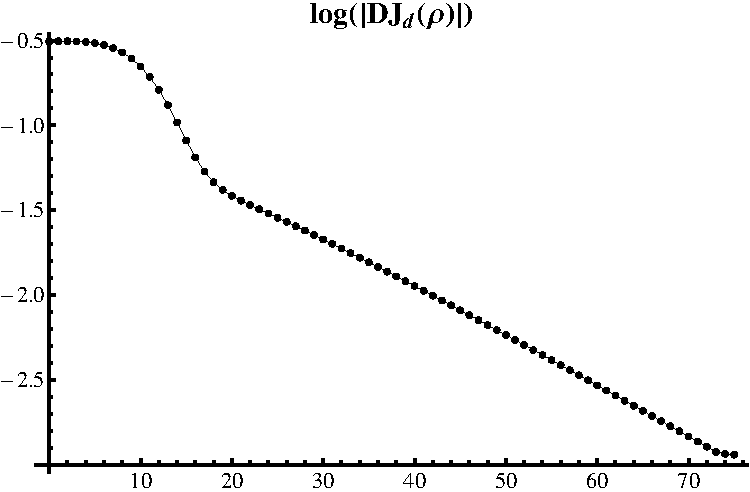
\includegraphics[width = 0.47\textwidth]{conv_12_links.pdf}
\caption{Convergence of steepest descent.}
\label{fig-conv}
\end{wrapfigure}

For the example, optimally identifying a 12-link  (31 configuration, 62 state) model from 20 seconds of manipulation activity (2000 data points recorded at 100Hz) takes 219.05 minutes on a Macbook air.  For comparison, we also identified a 6-link (19 configuration 38 state) model.  It converged nearly four times quicker, in 61.01 minutes, but the optimal cost was higher at $J_d = 1.54588$.  The design tradeoff is between model fidelity and computation time.

In the full paper we will extend these results to multiple experiments as discussed in Section \ref{sec-tech}


\section{Experiments}
\label{sec-exps}
\begin{figure*}
\centering
\def\svgwidth{.9\textwidth}
\input{three_bloops.pdf_tex}
\caption{Three distinct configurations along with snapshots of the physical system.  \textbf{a)} The frames for Baxter and the loop in their initial configuration. \textbf{b)} Baxter ``twisting'' the loop. \textbf{c)} Baxter ``bending'' the loop.}
\label{fig-3bloops}
\end{figure*}
\begin{wrapfigure}{r}{0.4\textwidth}
\centering
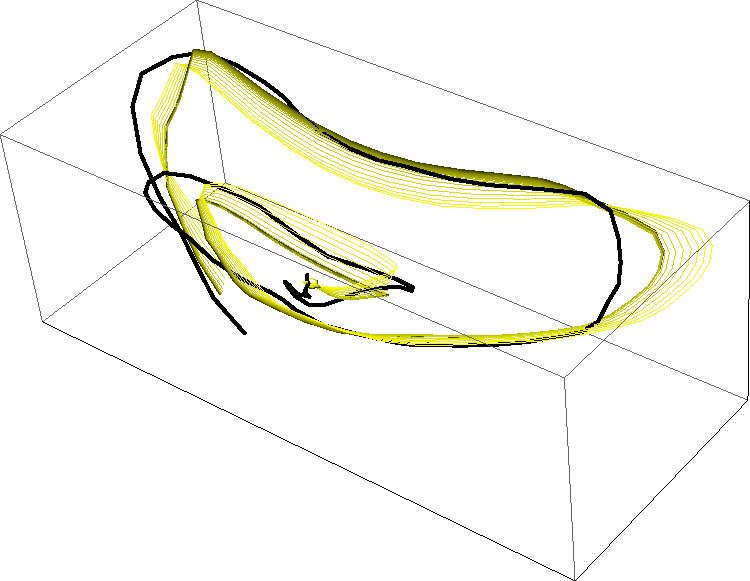
\includegraphics[width = 0.37\textwidth]{paths12.pdf}
\caption{The path the robot's end effector took through space.  The black line is the measured end effector's path while the yellow lines are the end effector's simulated path for each iteration of the steepest descent algorithm.  The iteration numbers are ordered from lighter yellow to darker yellow.  }
\label{fig-paths}
\end{wrapfigure}
The experiment is set up as follows.  We use Rethink Robotics' Baxter robot \cite{guizzo2011rethink}, shown in Figure~\ref{fig-baxter_image_1}, to manipulate and measure an inflated rubber loop (bicycle tyre). Baxter's arm is positioned similarly to that in Figure~\ref{fig-baxter_image_1}.  The top of the loop is placed in Baxter's gripper and the bottom is clamped to the table.   The loop is initially positioned vertically. The loop has a radius of $0.355$ meters and a mass of $0.132$ kilograms.  The arm is run through a recorded motion that is designed to stretch, bend, and twist the tube. The arm's joint angles and torques are captured and recorded every 100Hz.  The measured joint angles have a position resolution of +/- 5 mm.  The process of ``playing'' a recorded motion and recording the joint angles and torques constitutes a single experiment.

In order to improve the identification, multiple experiments are conducted.  These experiments may include manipulating the loop with two arms instead of one or use the second arm to "probe" whether the tube is where the model estimates it should be.  This estimate will worsen the greater the loop is twisted or bent, but the amount it will be off will depend on the quality of the identification.

Images of baxter manipulating the loop compared to the simulated system is shown in Figure~\ref{fig-3bloops}.  For this simulation, the loop is composed of 12 links.  The simulation is dependent on the stiffness values of the loop.  The identification goal is to find the stiffness properties which correspond to a simulation that best matches the measured data.  The results of optimally identifying the loop's stiffness parameters for a single experiment are shown in Figure~\ref{fig-paths}.  The figure compares the measured end effector path with the simulated end effector path for each iteration of a steepest descent.  We extend this result in the full paper to multiple parameters.



%``We are using a flexible loop as a running example throughout the paper.  We assume the robot has already rigidly grasped the object at one end and that it is clamped at the other. The robot then bends, twists, and stretches the loop.  During the manipulation, the robot measures the arm's joint torques and joint angles.  With this information, it is possible to back out mechanical properties of the loop in order to generate an accurate model for future control and manipulation.''

%``The experiment is set up as follows. Baxter’s arm is positioned similarly to that in Figure 1. The top of an inflated rubber loop (bicycle tyre) is placed in Baxter’s gripper and the bottom is clamped to the table. The loop is initially positioned vertically. The loop has a radius of 0.355 meters and a mass of 0.132 kilograms. The arm is run through a recorded motion that is designed to stretch, bend, and twist the tube. The arm’s joint angles and torques are captured every 100Hz, which we compile into the two vectors bmeas(t) and Tmeas(t). The measured joint angles have a position resolution of +/- 5 mm.
%The measured joint angles bmeas correspond to a subset of the system configuration q, where the remaining config- urations belong to the loop. We label this subset of q that describes the arm as b. The optimization goal is to choose model parameters so that |b − bmeas| is small.''

%``We use Rethink Robotics' Baxter \cite{guizzo2011rethink} robot to both manipulate and measure the loop.  Each of Baxter's arms have 7 degrees of freedom.  The arms are designed for compliance since each joint has series elastic actuators that allows for force sensing and control.  A picture of Baxter manipulating rubber loop is in Figure~\ref{fig-baxter_image_1}.''


\section{Main Experimental Insights}
Through the proposed parameter identification procedure, we calculate the model parameters that best match physical phenomena within the constraint of the chosen model.  This process is important since an improved model can make for better object manipulation.  However, it is unclear what this matching tells us about the object's physical properties.  Certainly, measuring at a single contact point provides little insight into the interior stress and strain of the rubber loop.

When a flexible object does not have uniform stiffness, multiple experiments are needed at different contact points to identify the non-uniformity.  Also, objects with more complex geometries require additional experiments.  For instance, grasping and manipulating a single leaf of a tomato plant provides little insight to identify the full plant.

As the parameter identification process is informed from actual manipulation, the proposed method could also be used online, thereby improving a model estimate with the time the robot spent with an object growing. We note that identification in this paper relies on proprioceptive data compared with model prediction. Other directions for identification are: (1) using proprioception of a second arm to validate hypotheses on object movement and obtaining additional measurements and constraints, and (2) combine this data with exterioperception such as cameras, 3D data, and dynamic tactile sensing \cite{hughes2014}. 

Finally, we note that the fidelity of the approach heavily depends on the choice of the model. While this choice strongly depends on the desired manipulation task, we are also interested in automatically finding appropriate model representations for given geometries and conceptual knowledge on the object, such as ``plant'', ``tube'' or ``sheet'', e.g.  


\bibliographystyle{plain}
\bibliography{abstract-ISER_cites}

\end{document}
